\documentclass{standalone}
\usepackage{pgfplots}
\pgfplotsset{compat=1.17}

\begin{document}

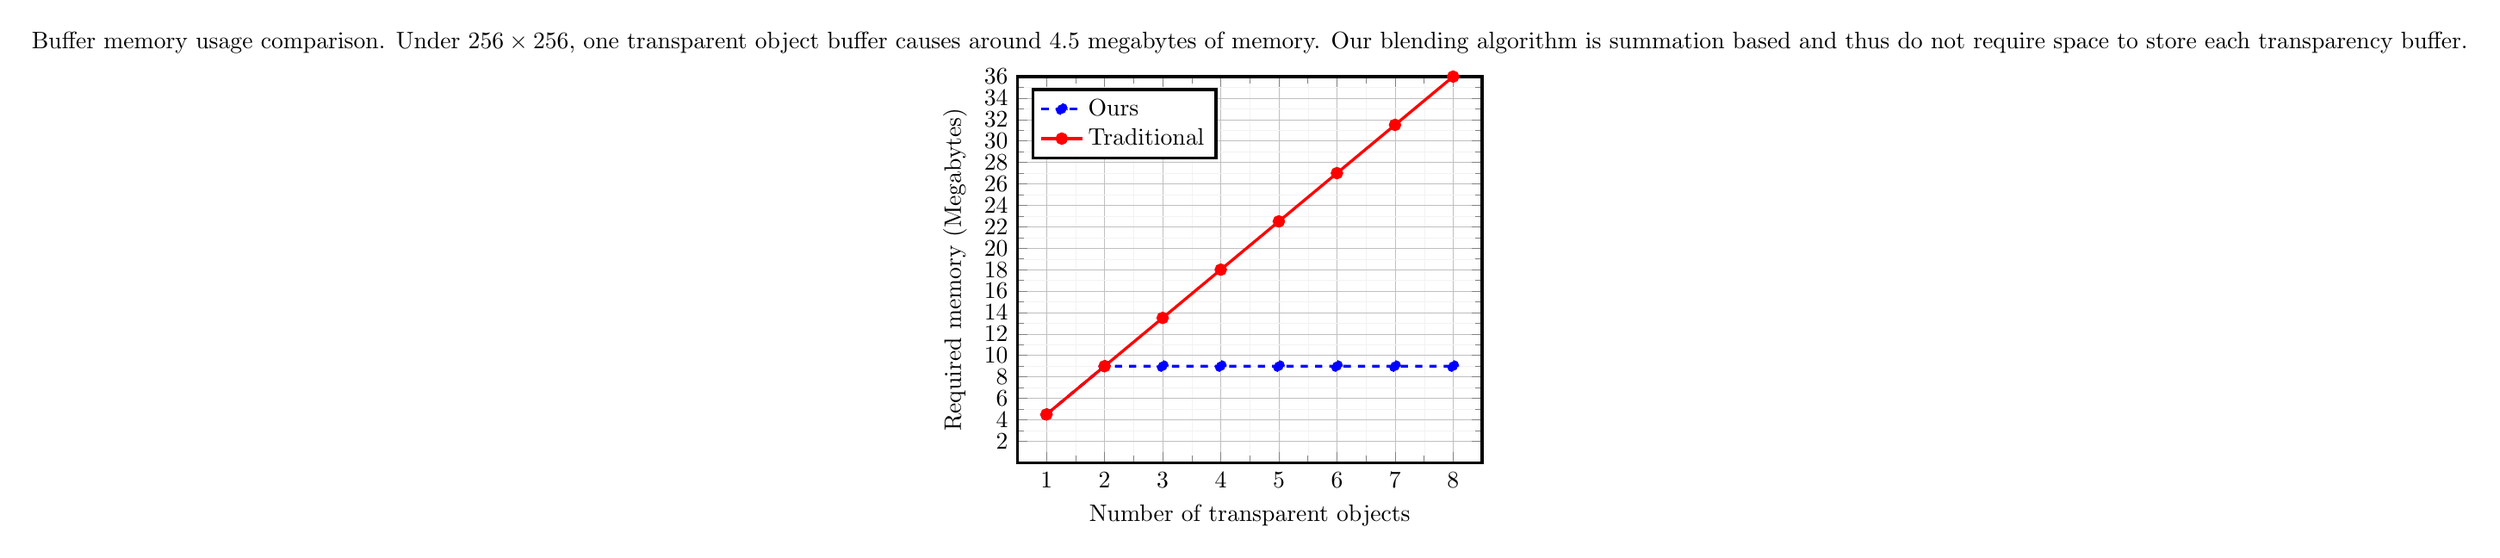
\begin{tikzpicture}
    \begin{axis}[
        title={Buffer memory usage comparison. Under $256 \times 256$, one transparent object buffer causes around 4.5 megabytes of memory. Our blending algorithm is summation based and thus do not require space to store each transparency buffer.},
        xlabel={Number of transparent objects},
        ylabel={Required memory (Megabytes)},
        xmin=0.5, xmax=8.5,
        ymin=0, ymax=36,
        xtick={1,2,3,4,5,6,7,8},
        ytick={2,4,6,8,10,12,14,16,18,20,22,24,26,28,30,32,34,36},
        grid=both,
        grid style={line width=.1pt, draw=gray!10},
        major grid style={line width=.2pt,draw=gray!50},
        minor tick num=1,
        enlargelimits=false,
        legend pos=north west,
        legend cell align=left,
        style={line width=1.2pt},
        samples=2
    ]
        
        % Plot "Ours" data (blue line)
        \addplot[mark=*, blue, dashed] coordinates {
            (1, 4.5)
            (2, 9)
            (3, 9)
            (4, 9)
            (5, 9)
            (6, 9)
            (7, 9)
            (8, 9)
        };
        \addlegendentry{Ours}
        
        % Plot "Traditional" data (red line)
        \addplot[mark=*, red] coordinates {
            (1, 4.5)
            (2, 9)
            (3, 13.5)
            (4, 18)
            (5, 22.5)
            (6, 27)
            (7, 31.5)
            (8, 36)
        };
        \addlegendentry{Traditional}
        
    \end{axis}
\end{tikzpicture}

\end{document}